\documentclass[10pt]{beamer}

% =========================
% Theme (sobre / académique)
% =========================
\usetheme{Madrid}
\usecolortheme{default}
\usefonttheme{professionalfonts}
\setbeamertemplate{navigation symbols}{}
\setbeamertemplate{footline}[frame number]

% =========================
% Packages
% =========================
\usepackage[utf8]{inputenc}
\usepackage[T1]{fontenc}
\usepackage{lmodern}
\usepackage{graphicx}
\usepackage{amsmath}
\usepackage{tikz}
\usetikzlibrary{shapes}

% =========================
% Meta
% =========================
\title[Model-Based Digital Twin]{Démarrer le post-doctorat\\Model-Based Digital Twin\\sous les meilleurs auspices}
\author{Julien Soulé}
\institute{Candidature Post-doctorat -- LIST}
\date{\today}

% =========================
\begin{document}
% =========================

% -------------------------
\begin{frame}
    \titlepage
\end{frame}

% -------------------------
\begin{frame}{Intention et positionnement}
    \textbf{Objectif de cette présentation}
    \begin{itemize}
        \item Présenter une compréhension synthétique du cadre \textit{model-based / model-driven}
        \item Proposer une projection opérationnelle pour contribuer dès les premiers mois
    \end{itemize}

    \vspace{0.3cm}
    \textbf{Positionnement scientifique et ingénierie}
    \begin{itemize}
        \item Approche \textit{model-based system engineering}
        \item Centralité des \textbf{modèles de conception explicites}
        \item Simulations et outils numériques comme \textbf{supports maîtrisés} de l’analyse et de l’aide à la décision
    \end{itemize}
\end{frame}

% -------------------------
\begin{frame}{Lecture du projet et du cadre model-based}
    \textbf{Lecture synthétique du pipeline Digital Twin}

    \vspace{0.2cm}
    \begin{center}
        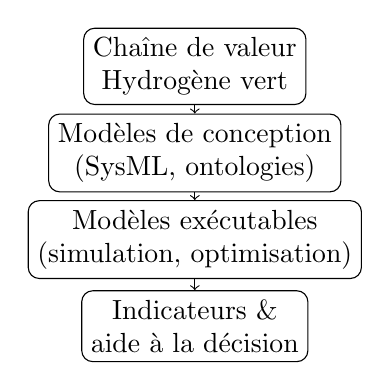
\begin{tikzpicture}[node distance=1.1cm, every node/.style={draw, rectangle, rounded corners, align=center}]
            \node (a) {Chaîne de valeur\\Hydrogène vert};
            \node (b) [below of=a] {Modèles de conception\\(SysML, ontologies)};
            \node (c) [below of=b] {Modèles exécutables\\(simulation, optimisation)};
            \node (d) [below of=c] {Indicateurs \&\\aide à la décision};

            \draw[->] (a) -- (b);
            \draw[->] (b) -- (c);
            \draw[->] (c) -- (d);
        \end{tikzpicture}
    \end{center}

    \vspace{0.2cm}
    \begin{itemize}
        \item Les modèles de conception constituent le \textbf{socle structurant} du Digital Twin
        \item Les modèles exécutables permettent l’\textbf{exploration} et l’\textbf{analyse} de scénarios dans un cadre contrôlé
        \item Les résultats sont interprétés au regard des \textbf{hypothèses} et \textbf{abstractions} initiales
    \end{itemize}
\end{frame}

% -------------------------
\begin{frame}{Apports concrets à court terme (0--6 mois)}
    \textbf{Axes de contribution prioritaires}

    \vspace{0.1cm}
    \begin{enumerate}
        \item \textbf{Structuration des modèles}
              \begin{itemize}
                  \item Clarification des concepts, frontières du système, et points de vue
                  \item Formalisation progressive et cohérente (structurel / comportemental)
                  \item Alignement des modèles avec les hypothèses métier
              \end{itemize}

              \vspace{0.15cm}
        \item \textbf{Prototypes orientés ingénierie}
              \begin{itemize}
                  \item Modèles exécutables à des fins d’analyse (reproductibilité, traçabilité)
                  \item Chaînes de simulation évolutives et documentées
                  \item Visualisation et interfaces facilitant l’appropriation par les acteurs
              \end{itemize}

              \vspace{0.15cm}
        \item \textbf{Exploitation raisonnée des simulations}
              \begin{itemize}
                  \item Paramétrisation guidée par les modèles
                  \item Indicateurs explicables (qualitatifs / quantitatifs) pour l’aide à la décision
                  \item Validation et itérations sur les hypothèses
              \end{itemize}
    \end{enumerate}
\end{frame}

% -------------------------
\begin{frame}{Méthodologie de travail proposée}
    \textbf{Démarche model-driven itérative}

    \vspace{0.15cm}
    \begin{center}
        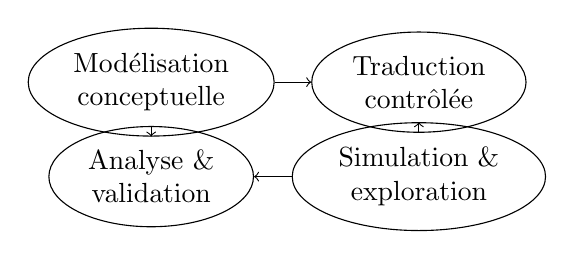
\begin{tikzpicture}[node distance=1.2cm, every node/.style={draw, ellipse, align=center}]
            \node (m1) {Modélisation\\conceptuelle};
            \node (m2) [right of=m1, xshift=2.2cm] {Traduction\\contrôlée};
            \node (m3) [below of=m2] {Simulation \&\\exploration};
            \node (m4) [left of=m3, xshift=-2.2cm] {Analyse \&\\validation};

            \draw[->] (m1) -- (m2);
            \draw[->] (m2) -- (m3);
            \draw[->] (m3) -- (m4);
            \draw[->] (m4) -- (m1);
        \end{tikzpicture}
    \end{center}

    \vspace{0.15cm}
    \textbf{Principes directeurs}
    \begin{itemize}
        \item Incrémentalité et cohérence inter-modèles
        \item Co-construction avec les experts (validation continue)
        \item Capitalisation : méthodologie, artefacts, documentation
    \end{itemize}
\end{frame}

% -------------------------
\begin{frame}{Projection scientifique et technique}
    \textbf{Contributions envisageables}
    \begin{itemize}
        \item Méthodologies model-based pour Digital Twins complexes
        \item Articulation entre modèles de conception et simulations
        \item Aide à la décision : indicateurs, traçabilité, explicabilité
    \end{itemize}

    \vspace{0.25cm}
    \textbf{Ouvertures maîtrisées}
    \begin{itemize}
        \item Optimisation et méthodes d’approximation lorsque pertinentes
        \item Approches data-driven \textbf{strictement encadrées par les modèles}
    \end{itemize}

    \vspace{0.25cm}
    \begin{block}{Principe directeur}
        Préserver la cohérence, la traçabilité et l’explicabilité sur l’ensemble du cycle de vie du Digital Twin.
    \end{block}
\end{frame}

% -------------------------
\begin{frame}{Motivation et conclusion}
    \textbf{Motivation}
    \begin{itemize}
        \item Cohérence avec mon parcours en modélisation / simulation de systèmes complexes
        \item Intérêt fort pour la transition énergétique et les enjeux industriels associés
        \item Volonté de contribuer durablement aux activités model-based du LIST
    \end{itemize}

    \vspace{0.3cm}
    \textbf{Conclusion}
    \begin{itemize}
        \item Contribution rigoureuse, progressive et immédiatement opérationnelle
        \item Alignement avec une approche \textit{model-based / model-driven}
        \item Base solide pour des résultats scientifiques et applicatifs
    \end{itemize}
\end{frame}

% -------------------------
\end{document}
